\documentclass[aspectratio=169]{beamer}
\usefonttheme{serif}
\usepackage{xeCJK}
\usepackage{fontspec}
\usepackage{graphicx}
\usepackage{listings}
\usepackage{xcolor}
\usepackage{indentfirst}
\usepackage{tikz}
\usepackage{amssymb}
\usepackage{amsthm}
\usepackage{amsmath}
\usepackage{tabularx}
\usepackage{hyperref}
\usepackage{ulem}
\usepackage{version}
\usepackage{thmtools}
\usepackage{qtree}
\usepackage{algpseudocode}
\usepackage{mathtools}
\usepackage{multicol}
\usepackage{xcolor}

\AtBeginDocument{%
    \DeclareSymbolFont{pureletters}{T1}{lmr}{\mddefault}{it}%
}

\XeTeXlinebreaklocale "zh"
\XeTeXlinebreakskip = 0pt plus 1pt

\setCJKmainfont{NotoSansTC-Medium.otf}
\setmainfont{JetBrainsMono-SemiBold.ttf}
\usetikzlibrary{arrows,decorations.markings,decorations.pathreplacing}
\newenvironment{Hint}{\noindent\textbf{Hint.}}{}

\tikzstyle {graph node} = [circle, draw, minimum width=1cm]
\tikzset{edge/.style = {decoration={markings,mark=at position 1 with %
            {\arrow[scale=2,>=stealth]{>}}},postaction={decorate}}}

\lstset{
    basicstyle=\ttfamily\normalsize,
    numberstyle=\normalsize,
    numbers=left,
    stepnumber=1,
    numbersep=3pt,
    commentstyle=\color{black!50},
    keywordstyle=\color{white!0!blue},
    stringstyle=\color{black!50!green},
    showspaces=false,
    showstringspaces=false,
    showtabs=false,
    tabsize=4,
    captionpos=b,
    breaklines=true,
    breakatwhitespace=false,
    escapeinside={\%*}{*)},
    morekeywords={*}
}

\AtBeginSection[]{
  \begin{frame}
  \vfill
  \centering
  \begin{beamercolorbox}[sep=8pt,center,shadow=true,rounded=true]{title}
    \usebeamerfont{title}\insertsectionhead\par%
  \end{beamercolorbox}
  \vfill
  \end{frame}
}

\title{DP}
\author{Koying}
\subtitle{SCIST x NHDK x 南 11 校寒訓 - 資言資語}
\date{2023-02-02}

\usetheme{Madrid}
\usecolortheme{default}
\setbeamertemplate{itemize items}[square]
\setbeamertemplate{enumerate items}[default]
\setbeamertemplate{blocks}[default]
\lstdefinestyle{myStyle}{
    belowcaptionskip=1\baselineskip,
    breaklines=true,
    frame=none,
    numbers=none, 
    basicstyle=\footnotesize\ttfamily,
    keywordstyle=\bfseries\color{green!40!black},
    commentstyle=\itshape\color{purple!40!black},
    identifierstyle=\color{blue},
    backgroundcolor=\color{gray!10!white},
}

\begin{document}

    \begin{frame}
        \titlepage
    \end{frame}

    \begin{frame}
        
\includegraphics[width=\textwidth]{./img/SCIST_Sponser.png}
    \end{frame}

    \begin{frame}{協辦單位:ITSA}
        \begin{center}
            
\includegraphics[width=0.5\textwidth]{./img/ITSA.png}
        \end{center}
    \end{frame}


    \begin{frame}{目錄}
        \begin{itemize}
            \item DP 入門
            \item DP 實作
            \item 線性 DP
            \item 背包問題
            \item 子序列 DP
            \item DAG DP
            \item 樹 DP
        \end{itemize}
    \end{frame}

    \section{DP 入門}

    \begin{frame}{DP 入門}
        \begin{itemize}
            \item DP (Dynamic Programming),動態規劃
            \item 利用將問題拆解成子問題的方式來解決問題
            \item 有些人可能聽過分治,同樣也是將問題拆解為子問題,比較不一樣的是 DP 主要是利用「記憶化的方式」,將許多會重複用到的子問題記錄下來
            \item DP 問題經常會有「最佳子結構」、「重疊子問題」兩大特徵
            \item 簡單用一句話來形容 DP 在做的事,便是將各種會用到多次,且最符合我們需要的答案記錄下來,以供之後使用,有點像是進階版的建表
        \end{itemize}
    \end{frame}

    \begin{frame}{DP 入門}
        \begin{block}{費氏數列}
            求出 $F_n \bmod 10^9 + 7\ (n \le 10^6)$
        \end{block}

        \begin{itemize}
            \item<1-> 以一般遞迴式的方式,我們會得到一個 $\mathcal{O}(2^n)$ 的複雜度,顯然是不符合我們的需求
            \item<2-> 如果將遞迴過程畫成一顆樹,會發現我們重複計算了很多「早就被算過」的東西
            \item<3-> 如果能夠將已經算過的東西記錄下來,就能夠用「空間」換取大量的「時間」
            \item<4-> 這便是 DP 最經典的「重疊子問題」例子。而以空間換取時間的做法,則被稱為「記憶化搜索」
        \end{itemize}
    \end{frame}

    \begin{frame}{國中數學}
        \begin{block}{路徑問題}
            給一個 $n \times m$ 的方格,求從左上角走到右下角的路徑數,且每步只能往右或往下走
        \end{block}

        \begin{itemize}
            \item<1-> 相信有認真上課的學員都知道,這題就是將原點設為 1,然後對於每個點 $i, j$,寫上 $i - 1, j$、$i, j - 1$ 兩個點的和
            \item<2-> 其實這就是動態規劃!
            \item<3-> \sout{OK,學校都已經教過了,今天的課就到這邊}
        \end{itemize}
    \end{frame}

    \begin{frame}{小試身手}
        \begin{block}{\href{https://cses.fi/problemset/task/1638}{Grid Paths}}
            路徑問題,有障礙物的版本
        \end{block}
    \end{frame}

    \section{DP 的組成與實作}

    \begin{frame}{DP 的兩大要素}
        \begin{itemize}
            \item<1-> DP 的運作過程由「狀態」、「轉移式」組成
            \item<2-> 「狀態」指的是利用陣列在紀錄子問題答案時,其 index 所代表的意義
            \item<2-> 而「轉移式」代表的則是大的狀態與小的狀態之間的關係
            \item<3-> 以剛剛的費氏數列為例子,我們會將狀態定義為:$dp_i$ 為費氏數列的第 $i$ 項
            \item<3-> 而「轉移式」便是大家熟知的:$dp_i = dp_{i - 1} + dp_{i - 2}$
            \item<4-> 這樣看似齊全了,但直接執行的話,會造成無限遞迴,因此我們還需要設計一個「邊界條件」,在這個例子便是 $dp_0 = 0, dp_1 = 1$
        \end{itemize}
    \end{frame}


    \begin{frame}{DP 的實作方式}
        \begin{itemize}
            \item 想要算出最終的狀態,主要有兩種方式:
            \begin{enumerate}
                \item Top down:從最終狀態 $(F_n)$,利用遞迴往回推
                \item Bottom up:從初始狀態 $(F_0)$,利用迴圈往前算,直到算到最終狀態
            \end{enumerate}
            \item 至於為什麼這樣命名呢?如果我們將遞迴樹畫出來,便可很簡單的發現其端倪了!
        \end{itemize}
    \end{frame}
    
    \begin{frame}{Top down 的特性}
        \begin{itemize}
            \item 只要推出轉移式與初始狀態,便可很教直觀的寫出程式碼
            \item 在某些情況可能會遞迴過深
            \item 遞迴常數較大,要注意可能會造成效能損失
            \item 範例程式碼:Top Down.cpp
        \end{itemize}
    \end{frame}


    \begin{frame}{Bottom up 的特性}
        \begin{itemize}
            \item 子問題需比母問題早算出,因此需要想好迴圈的順序
            \item 若將各個狀態與其轉移點的關係畫成一張圖,則迴圈的順序便是圖論中的「拓樸排序」
            \item 速度快,除了省去了遞迴常數之外,也經常能因 CPU 的快取機制獲得一部分的效能提升
            \item 範例程式碼:Bottom up.cpp
        \end{itemize}
    \end{frame}

    \section{前綴和}

    \begin{frame}{前綴和}
        \begin{itemize}
            \item<1-> 覺得 DP 很遙遠嗎?
            \item<2-> 其實你們都已經會了!
            \item<3-> 其實前綴和就是一個簡單的 DP 問題
            \item<4-> $dp_i$ 為 $a_1 \sim a_i$ 的總和,轉移式就是 $dp_i = dp_{i - 1} + a_i$
            \item<5-> 那如果是二維呢?
        \end{itemize}
    \end{frame}

    \begin{frame}{二維前綴和 - 排容}
        \begin{itemize}
            \item<1-> 狀態:$dp_{i, j}$ 為 $\displaystyle\sum_{k = 1}^{i}{\sum_{l = 1}^{j}{a_{i, j}}}$ 
            \item<2-> 如何轉移呢?相信大家國中時都學過一個公式:$(a + b)^2 = a^2 + b^2 + ab + ba$
            \item<3-> 這個公式便是利用排容原理,將重疊的部分扣除
            \item<3-> 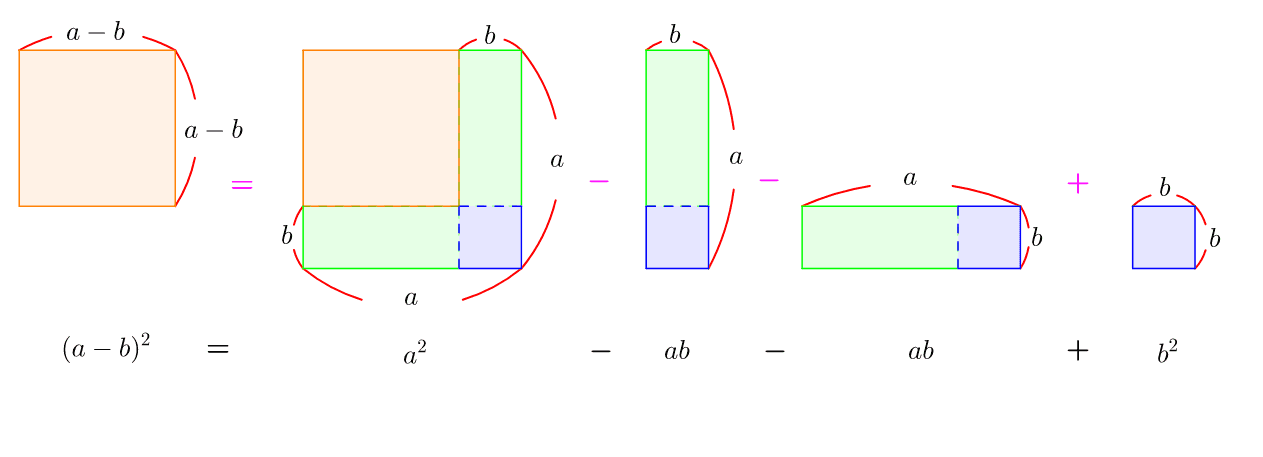
\includegraphics[width=\textwidth]{img/和平方公式.png}
        \end{itemize}
    \end{frame}

    \begin{frame}{二維前綴和 - 排容}
        \begin{itemize}
            \item<1-> 那簡單!我們的轉移式就也用排容來算就好了
            \item<2-> $dp_{i, j} = \begin{cases}
                0 & i = 0 \text{ or } j = 0 \\
                dp_{i - 1, j} + dp_{i, j - 1} - dp_{i - 1, j - 1} + a_{i, j} & \text{otherwise}
            \end{cases}$
            \item<3-> 那如果我們要求出 $(x1, y1), (x1, y2), (x2, y1), (x2, y2)$ 這塊矩形的總和,一樣使用排容原理即可
            \item<4-> $dp_{x2, y2} - dp_{x1 - 1, y2} - dp_{x2, y1 - 1} + dp_{x1 - 1, y1 - 1}$
        \end{itemize}
    \end{frame}

    \section{滾動優化}

    \begin{frame}{滾動 DP}
        \begin{block}{\href{https://cses.fi/problemset/task/1638}{Grid Paths}}
            路徑問題,有障礙物的版本
        \end{block}

        \begin{itemize}
            \item<1-> 我們回到剛剛那題 Grid Path
            \item<2-> 觀察後可以發現,$dp_i$ 的轉移點都是在 $dp_{i - 1}$
            \item<2-> 代表 $dp_1 \sim dp_{i - 2}$ 都是沒用的
            \item<3-> 那我們何不省點空間呢?
        \end{itemize}
    \end{frame}

    \begin{frame}{滾動 DP}
        \begin{block}{\href{https://cses.fi/problemset/task/1638}{Grid Paths}}
            路徑問題,有障礙物的版本
        \end{block}

        \begin{itemize}
            \item<1-> 既然只用到兩列,那我們陣列就只開兩列 dp[0]、dp[1]
            \item<2-> 當 $i \equiv 0 \pmod{2}$ 時,就使用 dp[0],反之 dp[1]
            \item<2-> 這樣就可以將空間複雜度降到 $n$ 了!
            \item<3-> 需要注意的是,陣列中可能還存著以前的資訊,所以要先記得初始化
            \item<4-> 一些小技巧:
            \begin{itemize}
                \item<4-> 偶 0 奇 1:$i \& 2$
                \item<4-> 偶 1 奇 0:$i \^ 1$
            \end{itemize}
        \end{itemize}
    \end{frame}


    \section{線性 DP}

    \begin{frame}{線性 DP}
        \begin{block}{\href{https://atcoder.jp/contests/dp/tasks/dp_a}{AtCoder DP Contest A - Frog 1}}
            每顆石頭的高度為 $h_i$,從第 $i$ 顆跳到第 $j$ 顆的代價是 $\lvert h_i - h_j \rvert$ 每次可以跳 $1$ 或 $2$ 格,求從第 $1$ 格跳到第 $N$ 格的最小代價
        \end{block}

        \begin{itemize}
            \item<1-> 首先我們先訂定狀態:$dp_i$ 為目前停在第 $i$ 格的最小代價
            \item<2-> 經由題目可知,第 $i$ 格可由第 $i - 1, i - 2$ 格得來,因此 $i - 1, i - 2$ 便是 $i$ 的「轉移點」
            \item<3-> 有了轉移點之後,我們就能夠推出轉移式:$dp_i = \min(dp_{i - 1} + \lvert h_{i} - h_{i - 1} \rvert, dp_{i - 2} + \lvert h_{i} - h_{i - 1} \rvert)$,
            而初始狀態則是:$dp_1 = 0, dp_2 = \lvert h_1 - h_2 \rvert$
            \item<4-> 時間複雜度 $\mathcal{O}(n)$
            \item<5-> 這種有關線性遞迴的 DP 便稱為「線性 DP」
            \item<6-> 
                $dp_i =
                \begin{cases}
                    0 & \text{if } i = 1 \\
                    \lvert h_1 - h_2 \rvert & \text{if } i = 2 \\
                    \min(dp_{i - 1} + \lvert h_{i} - h_{i - 1} \rvert, dp_{i - 2} + \lvert h_{i} - h_{i - 1} \rvert) & \text{otherwise}
                \end{cases}$
        \end{itemize}
    \end{frame}

    \begin{frame}{線性 DP}
        \begin{block}{\href{https://cses.fi/problemset/task/1633}{CSES Dice Combinations}}
            你有無限多顆六面骰,求丟出的點數總和為 $n$ 的方法數
        \end{block}

        \begin{itemize}
            \item<1-> 解決一些排列組合問題也是 DP 的其中一個用處
            \item<2-> 狀態應該不難訂:$dp_i$ 為丟出的點數總和為 $i$ 的方法數
            \item<3-> 觀察一下題目條件,可以發現當目前點數為 $i - 6 \sim i - 1$ 時,再丟一顆骰子,點數和就有機會變成 $i$
            \item<4-> 因此 $i - 1 \sim i - 6$ 便是 $i$ 的轉移點
            \item<5-> 最終轉移式:
            $dp_i = \begin{cases}
                1 & \text{ if } i = 0 \\
                \displaystyle\sum_{j = 1}^{i}{dp_i} & \text{ if } i \le 6 \\
                \displaystyle\sum_{j = i - 6}^{i - 1}{dp_i} & \text{ otherwise }
            \end{cases}$
        \end{itemize}
    \end{frame}

    \begin{frame}{例題}
        \begin{block}{\href{https://atcoder.jp/contests/dp/tasks/dp_a}{AtCoder DP Contest A - Frog 1}}
            每顆石頭的高度為 $h_i$,從第 $i$ 顆跳到第 $j$ 顆的代價是 $\lvert h_i - h_j \rvert$ 每次可以跳 $1$ 或 $2$ 格,求從第 $1$ 格跳到第 $N$ 格的最小代價
        \end{block}

        \begin{block}{\href{https://cses.fi/problemset/task/1633}{CSES Dice Combinations}}
            你有無限多顆六面骰,求丟出的點數總和為 $n$ 的方法數
        \end{block}

        \begin{block}{\href{https://atcoder.jp/contests/dp/tasks/dp_b}{AtCoder DP Contest B - Frog 2}}
            每顆石頭的高度為 $h_i$,從第 $i$ 顆跳到第 $j$ 顆的代價是 $\lvert h_i - h_j \rvert$ 每次可以跳 $1 \sim k$ 格,求從第 $1$ 格跳到第 $N$ 格的最小代價
        \end{block}

        \begin{block}{\href{https://toj.tfcis.org/oj/pro/470/}{2020 台南一中 x 台南女中聯合寒訓 pD. 公假無雙}}
            見原題
        \end{block}
    \end{frame}

    \begin{frame}{例題}
        \begin{block}{\href{https://atcoder.jp/contests/dp/tasks/dp_c}{AtCoder DP Contest C - Vacation}}
            每天有三種活動,每種活動都有一個分數,求相鄰兩天不為同一活動時的最大分數和
        \end{block}

        \begin{block}{\href{https://cses.fi/problemset/task/1637}{CSES Removing Digits}}
            給定一數字 $n$,每次可以減去 $n$ 的任意一位數字,求最少減幾次可以減到 $0\ (n \le 10^6)$ \\
            如:$27 \rightarrow 20 \rightarrow 18 \rightarrow 10 \rightarrow 9 \rightarrow 0$
        \end{block}

        \begin{block}{\href{https://codeforces.com/contest/1625/problem/C}{CF 1625C. Road Optimization}}
            一條長度為 $l$ 的道路上有 $n$ 個限速牌,每個限速牌上會寫著一個數字 $a_i$,
            代表車子以最高限速行駛時,每公里需要花 $a_i$,而車子經過該車速牌就會調整車速為限速牌上的最高時速。\\
            你可以移除最多 $k$ 個限速牌,求車子開過所需的最少時間
        \end{block}
    \end{frame}

    \section{背包問題}

    \begin{frame}{背包問題}
        \begin{itemize}
            \item 背包問題算是 DP 中最經典的題型,網路上直接搜尋動態規劃大概十篇有九篇都是背包問題
            \item 背包問題主要分為三種:
            \begin{enumerate}
                \item 0-1 背包問題:每種物品只有一個
                \item 無限背包問題:每種物品有無限個
                \item 有限背包問題:每種物品有有限個
            \end{enumerate}
            \item 今天的課程會提到前兩種(其實也是線性 DP 的變種)
        \end{itemize}
    \end{frame}

    \begin{frame}{0-1 背包問題}
        \begin{block}{\href{https://atcoder.jp/contests/dp/tasks/dp_d}{AtCoder DP Contest D - Knapsack 1}}
            有 $N$ 種物品,每種物品的重量為 $w_i$,價值為 $v_i$,背包的容量為 $W$,求背包裡的物品的最大價值\\
            $(N \le 100, W \le 10^5, w_i \le W, v_i \le 10^9)$
        \end{block}

        \begin{itemize}
            \item<1-> 題目問的是最多裝 $W$ 的最大價值,那我們就用重量當作狀態吧!$dp_i$ 代表重量為 $i$ 時的最大價值
            \item<2-> 對於重量 $i$,可以透過拿取第 $j$ 種物品讓重量變為 $i + w_j$,因此轉移點為 $i - w_j$
            \item<3-> 那我們就可以很輕鬆的推出轉移式了!
            \item<4-> $dp_i = \begin{cases}
                0 & \text { if } if < 0 \\
                \max(dp_i, dp_{i - w_j} + v_j) & \text { otherwise }
            \end{cases}$
            \item<5-> 實作小細節:由於要求最大價值,因此對於所有 $i > 0$,$dp_i$ 的初始值為 $-\infty$,最後答案便是最大的 $i$ 滿足 $dp_i > 0$
        \end{itemize}
    \end{frame}

    \begin{frame}{0-1 背包問題}
        \begin{block}{\href{https://atcoder.jp/contests/dp/tasks/dp_e}{AtCoder DP Contest E - Knapsack 2}}
            有 $N$ 種物品,每種物品的重量為 $w_i$,價值為 $v_i$,背包的容量為 $W$,求背包裡的物品的最小重量\\
            $(N \le 100, W \le 10^9, w_i \le W, v_i \le 10^3)$  
        \end{block}

        \begin{itemize}
            \item<1-> 可以發現 $W$ 最大來到了 $10^9$,因此我們需要更改狀態設計
            \item<2-> 除了重量,還有甚麼可以當作狀態呢?
            \item<3-> 觀察一下題目,發現最多裝 $W$ 的最大價值,可以轉換為最大價值且最多裝 $W$,因此可以換個方向,改以價值當作狀態
            \item<4-> $dp_i$ 代表價值 $i$ 時所需的最小重量
            \item<5-> $dp_i = \begin{cases}
                0 & \text { if } i = 0 \\
                \min(dp_i, dp_{i - v_j} + w_j) & \text { otherwise }
            \end{cases}$
            \item<6-> 初始狀態:$dp_i = \infty\ (i > 0)$,答案就是最大的 $i$ 滿足 $dp_i \le W$
        \end{itemize}
    \end{frame}

    \begin{frame}{無限背包問題}
        \begin{block}{\href{https://cses.fi/problemset/task/1634}{Minimizing Coins}}
            硬幣問題,有無限個面額為 $c_1, c_2, \dots, c_n$ 的硬幣,求湊出 $x$ 元的最少硬幣數量 $(n \le 100, x, c_i \le 10^6)$
        \end{block}

        \begin{itemize}
            \item<1-> 還記得貪心課講到的硬幣問題嗎?當面額不存在倍數關係時,就可以用 DP 來解決!
            \item<2-> 題目要問湊出 $x$ 的最少數量,那我們就用總和當作狀態
            \item<3-> $dp_i$ 為湊出 $i$ 元的最少硬幣數量
            \item<4-> $dp_i = \begin{cases}
                0 & \text { if } i = 0 \\
                \min(dp_i, dp_{i - c_j} + 1) & \text { otherwise }
            \end{cases}$
            \item<5-> 初始狀態:$dp_i = \infty\ (i > 0)$,答案就是 $dp_x$
        \end{itemize}
    \end{frame}

    \begin{frame}{跟排列組合有關的背包問題}
        \begin{block}{\href{https://cses.fi/problemset/task/1635}{CSES Coin Combinations I}}
            你有面額為 $c_1, c_2, \dots, c_n$ 的硬幣,求湊出 $x$ 元的方案數量,[1, 2, 3]、[1, 3, 2] 算是兩種 $(n \le 100, x, c_i \le 10^6)$
        \end{block}

        \begin{itemize}
            \item<1-> 狀態應該很明顯:$dp_i$ 為湊出 $i$ 元的方法數
            \item<2-> 轉移式:$dp_i = \begin{cases}
                1 & \text { if } i = 0 \\
                \sum_{j = 1}^n dp_{i - c_j} & \text { otherwise }
            \end{cases}$
            \item<3-> Trivial la!
        \end{itemize}
    \end{frame}

    \begin{frame}{跟排列組合有關的背包問題}
        \begin{block}{\href{https://cses.fi/problemset/task/1636}{CSES Coin Combinations II}}
            你有面額為 $c_1, c_2, \dots, c_n$ 的硬幣,求湊出 $x$ 元的方案數量,[1, 2, 3]、[1, 3, 2] 算是同一種 $(n \le 100, x, c_i \le 10^6)$
        \end{block}

        \begin{itemize}
            \item<1-> 多了排列算同一種的限制該怎麼辦?
            \item<2-> 我們觀察一下原本的轉移式會有甚麼問題
            \item<3-> 如果外層迴圈是 $1 \sim x$(價值),內層迴圈為 $1 \sim n$(面額),那麼就會發生重複計算的問題,如上所述
            \item<4-> 如何解決?簡單,將硬幣面額的順序固定
            \item<5-> 因此我們只需要將兩層迴圈替換就可以了!
        \end{itemize}
    \end{frame}

    \begin{frame}{例題}
        \begin{block}{\href{https://atcoder.jp/contests/dp/tasks/dp_d}{AtCoder DP Contest D - Knapsack 1}}
            有 $N$ 種物品,每種物品的重量為 $w_i$,價值為 $v_i$,背包的容量為 $W$,求背包裡的物品的最大價值\\
            $(N \le 100, W \le 10^5, w_i \le W, v_i \le 10^9)$
        \end{block}

        \begin{block}{\href{https://atcoder.jp/contests/dp/tasks/dp_e}{AtCoder DP Contest E - Knapsack 2}}
            有 $N$ 種物品,每種物品的重量為 $w_i$,價值為 $v_i$,背包的容量為 $W$,求背包裡的物品的最小重量\\
            $(N \le 100, W \le 10^9, w_i \le W, v_i \le 10^3)$  
        \end{block}

        \begin{block}{\href{https://cses.fi/problemset/task/1634}{Minimizing Coins}}
            硬幣問題,有無限個面額為 $c_1, c_2, \dots, c_n$ 的硬幣,求湊出 $x$ 元的最少硬幣數量 $(n \le 100, x, c_i \le 10^6)$
        \end{block}
    \end{frame}

    \begin{frame}{例題}
        \begin{block}{\href{https://cses.fi/problemset/task/1635}{CSES Coin Combinations I}}
            你有面額為 $c_1, c_2, \dots, c_n$ 的硬幣,求湊出 $x$ 元的方案數量,[1, 2, 3]、[1, 3, 2] 算是兩種 $(n \le 100, x, c_i \le 10^6)$
        \end{block}

        \begin{block}{\href{https://cses.fi/problemset/task/1636}{CSES Coin Combinations II}}
            你有面額為 $c_1, c_2, \dots, c_n$ 的硬幣,求湊出 $x$ 元的方案數量,[1, 2, 3]、[1, 3, 2] 算是同一種 $(n \le 100, x, c_i \le 10^6)$
        \end{block}

        \begin{block}{\href{https://cses.fi/problemset/task/1158}{Book Shop}}
            見原題
        \end{block}
    \end{frame}

    \begin{frame}{補充 - 有限背包問題}
        \begin{block}{有限背包問題}
            總共有 $n$ 種物品,每個物品有其數量 $c_i$、重量 $w_i$、價值 $v_i$,背包的容量為 $W$,求背包裡的物品的最大價值\\
            $(n \le 1000, c_i \le 10^9, w_i \le 100, W \le 1000)$
        \end{block}

        \begin{itemize}
            \item<1-> 注意物品數量不再是無限或是 0-1
            \item<2-> 如果將每個物品都拆開來看的話,光是物品數量就會超過 $10^9$
            \item<3-> 還記得二進位這東西嗎?我們只需要有 $2^0, 2^1, \dots, 2^n$,便可湊出 $0 \sim 2^{n + 1} - 1$
            \item<4-> 在這裡也同理!我們將 $c_i$ 拆成 $2^0, 2^1, \dots$,就可以將物品數量變為 $\log{c_i}$ 了!
            \item<5-> 最後,再將這些拆好的物品,做 0-1 背包問題即可,時間複雜度 $nW\log{c_i}$
            \item<6-> 之後如果你們有機會學到 DP 優化,會再將這個做法優化到更快
        \end{itemize}
    \end{frame}



    \section{更多例題}

    \begin{frame}{例題}
        \begin{itemize}
            \item \href{https://cses.fi/problemset/task/1746}{Array Description}
            \item \href{https://cses.fi/problemset/task/2413}{Counting Towers}
            \item \href{https://codeforces.com/problemset/problem/1526/C1}{CF 1526C1. Potions (Easy Version)}
        \end{itemize}
    \end{frame}

    \section{子序列 DP}

    \begin{frame}{一些名詞解釋}
        \begin{itemize}
            \item Subsequence 子序列:從一個字串中挑出幾個字元組成的字串,前後相對順序不變,如:$abc$ 的子序列為 $a, b, c, ab, ac, bc, abc$
            \item Substring 子字串:從一個字串中挑出某個區間的字元組成的字串,如:$abc$ 的子字串為 $a, b, c, ab, bc, abc$
        \end{itemize}
    \end{frame}

    \begin{frame}{LCS}
        \begin{itemize}
            \item<1-> LCS:Longest Common Subsequence,最長共同子序列
            \item<2-> 給定兩字串 $s_1, s_2$,求一個最長的字串長度,使得該字串為 $s_1, s_2$ 的子序列
        \end{itemize}
    \end{frame}

    \begin{frame}{LCS}
        \begin{itemize}
            \item<1-> 子序列 DP 的轉移式算是比較特別的
            \item<2-> $dp_{i, j}$:$s_1$ 的前 $i$ 個元素與 $s_2$ 的前 $j$ 個元素的 LCS 長度
            \item<3-> 怎麼轉移呢?可以觀察到,$s_{1, i}$ 與 $s_{2, j}$ 只有兩種關係:一樣 or 不一樣
        \end{itemize}
    \end{frame}

    \begin{frame}{LCS}
        \begin{itemize}
            \item<1-> 我們先來看 $s_{1, i} = s_{2, j}$ 的情況
            \item<2-> 假設 $s_{1, i} = s_{2, j}$,那麼以 $s_{1, i}$ 為結尾的某個共同子序列,
            去掉結尾之後,就會變成 $s_1$ 的前 $i - 1$ 個元素與 $s_2$ 的前 $j - 1$ 個元素的 LCS
            \item<3-> 例如:$s_1 = \text{abcd}$,$s_2 = \text{acd}$,
            而 $i = 4, j = 3$ 時,$s_{1, 4} = s_{2, 3}$,因此以 d 結尾的 LCS 就會是 "abc"、"ac" 的 LCS 加上 d
            \item<4-> 發現這些性質之後,我們就可以推出在這樣的情況,$dp_{i, j} = dp_{i - 1, j - 1} + 1$ 了!
        \end{itemize}
    \end{frame}

    \begin{frame}{LCS}
        \begin{itemize}
            \item<1-> 那假如不一樣呢?
            \item<2-> 因為 $s_{1, i} \neq s_{2, j}$,所以 $(i, j)$ 的 LCS 一定不會有 $s_{1, i}$ 或是 $s_{2, j}$
            \item<3-> 這代表 $i, j$ 都是沒用的!
            \item<4-> 既然他沒用,那我們就隨便抓之前的狀態當作最佳解吧!
            \item<5-> 在這個狀態下的轉移式:$dp_{i, j} = \max(dp_{i - 1, j}, dp_{i, j - 1})$
        \end{itemize}
    \end{frame}

    \begin{frame}{LCS}
        $$
        dp_{i, j} = \begin{cases}
            dp_{i - 1, j - 1} + 1 & \text{if } s_{1, i} = s_{2, j} \\
            \max(dp_{i - 1, j}, dp_{i, j - 1}) & \text{otherwise}
        \end{cases}
        $$
    \end{frame}

    \begin{frame}{LCS 構造解}
        \begin{itemize}
            \item<1-> 我們可以先來看看\href{https://web.ntnu.edu.tw/~algo/Subsequence2.html}{動畫}
            \item<2-> $s_{1, i} = s_{2, j}$:代表轉移點在 $(i - 1, j - 1)$
            \item<2-> 將答案 $ans$ 加上 $s_{1, i}$、i - 1、j - 1
            \item<3-> $s_{1, i} \neq s_{2, j}$:代表轉移點在 $(i - 1, j)$ 或是 $(i, j - 1)$
            \item<3-> 看哪個比較大,將 $i, j$ 移至該點
            \item<4-> 最後 $ans$ 的逆序就是答案!
        \end{itemize}
    \end{frame}

    \begin{frame}{LCS 例題}
        \begin{block}{\href{https://atcoder.jp/contests/dp/tasks/dp_f}{AtCoder DP Contest F. LCS}}
            給兩字串,求 LCS
        \end{block}
    \end{frame}

    \section{編輯距離}

    \begin{frame}{編輯距離}
        \begin{itemize}
            \item 對於兩個字串 $s_1, s_2$,你有以下三種方法可以操作:
            \begin{itemize}
                \item 刪除某個字元
                \item 插入某個字元
                \item 修改某個字元
            \end{itemize}
            \item 求需要最少操作幾次,才能將 $s_1$ 變成 $s_2$
            \item 操作次數稱為編輯距離
        \end{itemize}
    \end{frame}

    \begin{frame}{舉例}
        \begin{itemize}
            \item abc 可由一次刪除變成 ac
            \item abc 可由一次插入變成 abdc
            \item abc 可由一次修改變成 abd
        \end{itemize}
    \end{frame}

    \begin{frame}{轉移式}
        \begin{itemize}
            \item<1-> 提示:這邊的狀態定義跟 LCS 一樣,轉移式也跟 LCS 有異曲同工之妙
            \item<1-> $dp_{i, j}$ 為 $s_{1, 1} \dots s_{1, i}$ 跟 $s_{2, 1} \dots s_{2, j}$ 的編輯距離
            \item<1-> 試想可以怎麼從 LCS 的定義轉換過來
            \item<2-> $s_{1, i} = s_{2, j}$:顯然不需要在 $(i, j)$ 做任何操作
            \item<2-> 轉移式:$dp_{i, j} = dp_{i - 1, j - 1}$
        \end{itemize}
    \end{frame}

    \begin{frame}{轉移式 - 刪除}
        \begin{itemize}
            \item<1-> 接著是不同的情況
            \item<2-> 我們可以將 $s_{1, i}$ 刪除來得到 $s_{1, i - 1}$
            \item<2-> 也就是說,$(i, j)$ 可由一次編輯得到 $(i - 1, j)$ 的狀態
            \item<2-> $dp_{i, j} = dp_{i - 1, j} + 1$
        \end{itemize}
    \end{frame}

    \begin{frame}{轉移式 - 插入}
        \begin{itemize}
            \item<1-> 如果要在 $s_{1, i}$ 後插入一個字元,你會選哪個?
            \item<2-> 顯然:$s_{2, j}$,這樣才有意義
            \item<3-> 既然你要為了 $s_{2, j}$ 再插入一個字元使其相等,那為何不乾脆刪掉 $s_{2, j}$?
            \item<4-> 所以刪除等價於插入,轉移式相同
        \end{itemize}
    \end{frame}

    \begin{frame}{轉移式 - 修改}
        \begin{itemize}
            \item<1-> 修改後長度不變,但能夠滿足 $s_{1, i} = s_{2, i}$ 
            \item<2-> 而相等的情況我們剛剛討論過了,轉移點 $(i, j)$,只是這次需要花費一次編輯
            \item<3-> 轉移式:$dp_{i, j} = dp_{i - 1, j - 1} + 1$
        \end{itemize}
    \end{frame}

    \begin{frame}{最終轉移式}
        \begin{itemize}
            \item 最後,我們把三種情況的轉移式合併起來
            \item $$dp_{i, j} = \begin{cases}
            dp_{i - 1, j - 1} & s_{1, i} = s_{2, j} \\
            \min(dp_{i - 1, j - 1}, dp_{i - 1, j}, dp_{i, j - 1}) + 1 & \text{otherwise}
            \end{cases}$$
            \item 時間複雜度 $\mathcal{O}(n^2)$
        \end{itemize}
    \end{frame}

    \begin{frame}{例題}
        \begin{block}{\href{https://cses.fi/problemset/task/1639}{CSES Edit Distance}}
            編輯距離經典題
        \end{block}
    \end{frame}

    \begin{frame}{編輯距離}
        \begin{itemize}
            \item<1-> 編輯距離看起來好像很廢?
            \item<2-> 但他幫我完成了一份分數蠻高的探究與實作報告
            \item<3-> 事實上,編輯距離可用來計算兩個 DNA 的相似程度
            \item<4-> 如果你們有生物報告或是探究報告要做,可以參考一下 (O
        \end{itemize}
    \end{frame}

    \section{LIS}

    \begin{frame}{LIS}
        \begin{itemize}
            \item Longest Increasing Subsequence,最長遞增子序列
            \item 跟 LCS 一樣,都是子序列問題
            \item 只是從 "共同" 的子序列,變成一個字串裡最長且元素呈現遞增 $(s_i \le s_{i + 1})$ 的子序列
            \item 例如 16723 的 LIS 就是 123
        \end{itemize}
    \end{frame}

    \begin{frame}{$\mathcal{O}(n^2)$ 作法}
        \begin{itemize}
            \item<1-> 狀態定義:$dp_{i}$:以第 $i$ 個元素為結尾的 LIS
            \item<2-> 對於所有 $j < i$,如果 $s_{j} \le s_{i}$,那就代表 $s_{i}$ 可以接在 $s_{j}$ 後面
            \item<3-> 因此 $i$ 的轉移點就是對於所有 $j$,滿足 $j < i, s_{j} \le s_{i}$
            \item<4-> 取最好的接上去就可以了!
            \item<5-> $dp_{i} = \displaystyle\max_{j = 1}^{i - 1}(dp_{j} + 1),\ s_{j} \le s_{i}$
        \end{itemize}
    \end{frame}

    \begin{frame}{$\mathcal{O}(n\log{n})$ 作法} 
        \begin{itemize}
            \item<1-> $\mathcal{O}(n^2)$ 實在是太遜了,能不能更快?
            \item<2-> 遞增 $\Rightarrow$ 單調性 $\Rightarrow$ 能不能二分搜阿??
            \item<2-> 我們畫圖試試看,假設我們有 $\left\{ 4, 5, 1, 2, 3, 10, 7, 2 \right\}$
        \end{itemize}
    \end{frame}

    \begin{frame}{LIS}
        \begin{center}
            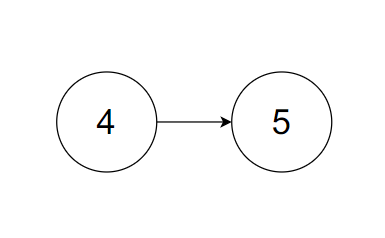
\includegraphics[width=0.4\textwidth]{img/LIS-1.png}
        \end{center}

        \begin{itemize}
            \item 一開始 $4, 5$ 都遞增,所以直接連起來
        \end{itemize}
    \end{frame}

    \begin{frame}{LIS}
        \begin{center}
            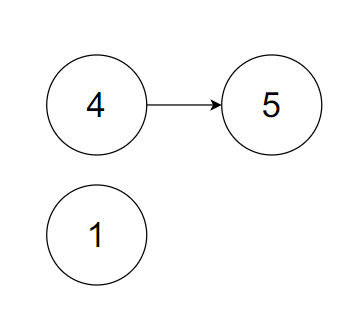
\includegraphics[width=0.4\textwidth]{img/LIS-2.png}
        \end{center}

        \begin{itemize}
            \item 接下來的 $1$ 比任何一個數字都還要小,因此我們先擺在旁邊
        \end{itemize}
    \end{frame}

    \begin{frame}{LIS}
        \begin{center}
            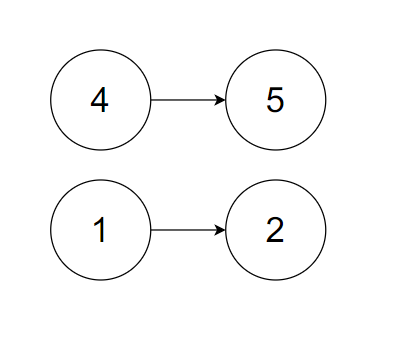
\includegraphics[width=0.4\textwidth]{img/LIS-3.png}
        \end{center}

        \begin{itemize}
            \item $2 > 1$,所以我們接在 $1$ 後面
        \end{itemize}
    \end{frame}

    \begin{frame}{LIS}
        \begin{center}
            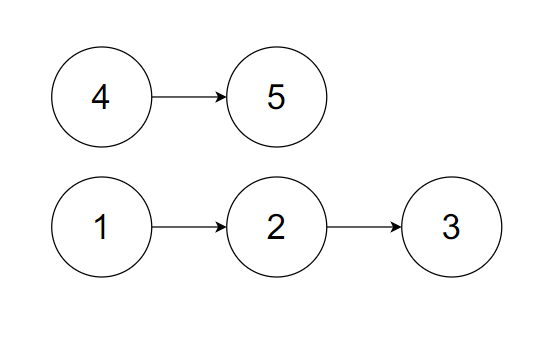
\includegraphics[width=0.4\textwidth]{img/LIS-4.png}
        \end{center}

        \begin{itemize}
            \item $3 > 2$,所以接在 $2$ 後面
            \item 可以發現,第二條鍊已經比第一條鍊長了,所以將第一條鍊捨棄
            \item 同樣位在第二位,$5 > 2$,顯然 $2$ 的潛力比較高(畢竟可以接比較多東西)
        \end{itemize}
    \end{frame}

    \begin{frame}{LIS}
        \begin{center}
            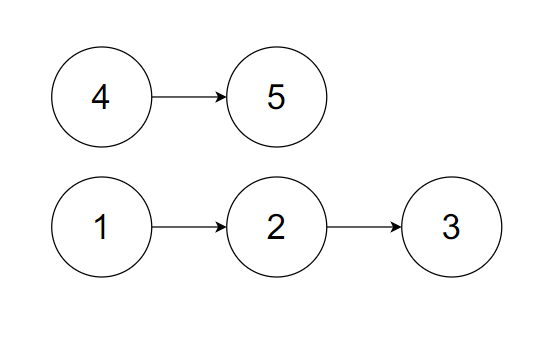
\includegraphics[width=0.4\textwidth]{img/LIS-4.png}
        \end{center}

        \begin{itemize}
            \item 換句話說,如果在兩條鍊的同一位有兩數字 $a, b$,且 $a > b$,那麼直接留下 $b$ 而不是 $a$ 肯定是最好的
            \item 也就是將數字大的直接淘汰
            \item 那我們重新試試看
        \end{itemize}
    \end{frame}

    \begin{frame}{LIS}
        \begin{center}
            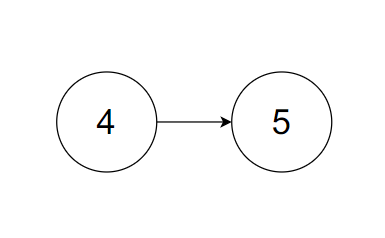
\includegraphics[width=0.4\textwidth]{img/LIS-5.png}
        \end{center}

        \begin{itemize}
            \item 這步驟一樣
        \end{itemize}
    \end{frame}

    \begin{frame}{LIS}
        \begin{center}
            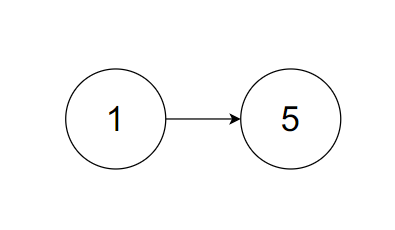
\includegraphics[width=0.4\textwidth]{img/LIS-6.png}
        \end{center}

        \begin{itemize}
            \item 原本 $1$ 應該是另一條鍊的第一項,但跟他並排的 $2 > 1$,潛力比較不好
            \item 所以我們把 $2$ 捨棄,填上 $1$
        \end{itemize}
    \end{frame}

    \begin{frame}{LIS}
        \begin{center}
            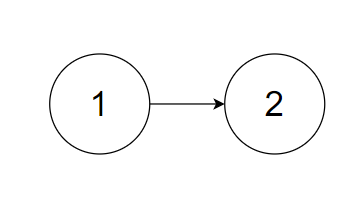
\includegraphics[width=0.4\textwidth]{img/LIS-7.png}
        \end{center}

        \begin{itemize}
            \item 再把 $5$ 用 $2$ 替換掉
        \end{itemize}
    \end{frame}

    \begin{frame}{LIS}
        \begin{center}
            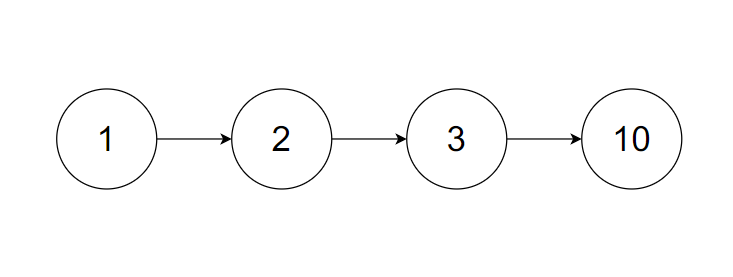
\includegraphics[width=0.4\textwidth]{img/LIS-8.png}
        \end{center}

        \begin{itemize}
            \item 將 $3, 10$ 接上
        \end{itemize}
    \end{frame}

    \begin{frame}{LIS}
        \begin{center}
            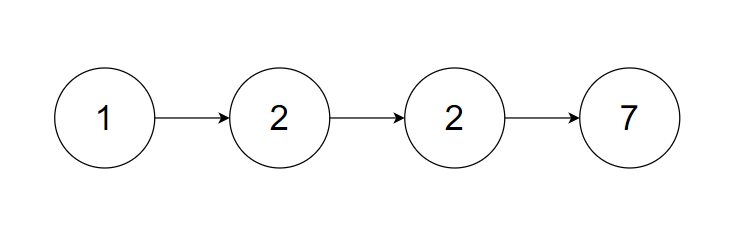
\includegraphics[width=0.4\textwidth]{img/LIS-9.png}
        \end{center}

        \begin{itemize}
            \item 依剛剛的規則,用 $7, 2$ 將 $10, 3$ 替換掉
            \item 最後得到的就是 LIS 長度了!
        \end{itemize}
    \end{frame}

    \begin{frame}{LIS}
        \begin{itemize}
            \item<1-> 觀察一下規則可以發現,當我們加入新元素 $A_i$ 時,我們可以在鍊裡找到一個元素 $A_j$ 並將其取代 ($A_j$ 滿足 $A_j \le A_i$ 且 $A_j$ 盡可能小)
            \item<2-> 有沒有很像二分搜?
            \item<3-> 其實這就是在做 lower bound
            \item<4-> 每次找到一個元素取代,若沒元素能夠取代就在鍊的尾端接上
            \item<5-> 時間複雜度 $\mathcal{O}(n\log{n})$
        \end{itemize}
    \end{frame}

    \begin{frame}{LIS}
        \begin{itemize}
            \item<1-> 應該有人有疑問:假設目前鍊長 $4$,我替換掉了位置 $2$,阿 $3, 4$ 又沒辦法接在 $2$ 後面,怎麼會合法?
            \item<2-> 這是因為這個鍊其實不是真正的 LIS,只是紀錄各種 IS 在同一位置上的最佳解罷了
            \item<3-> 你可以把他想像成是在 "新陳代謝"
        \end{itemize}
    \end{frame}

    \begin{frame}{子序列 DP 的構造解}
        \begin{itemize}
            \item<1-> 前面都是在講最大長度,沒有講構造出的答案
            \item<2-> DP 問題中,一個非常關鍵的點就是目前狀態的轉移點是哪一個
            \item<3-> 我們可以對每個狀態紀錄他是由哪個轉移點轉移得來的
            \item<3-> 最後再從最後一個一直往前推,就能夠找到答案了!
            \item<3-> 這部分就留給學員回家實作了
        \end{itemize}
    \end{frame}
    
    \begin{frame}{例題}
        \begin{block}{\href{https://cses.fi/problemset/task/1145}{CSES Increasing Subsequence}}
            LIS 經典題目
        \end{block}

        \begin{block}{\href{https://zerojudge.tw/ShowProblem?problemid=f608}{APCS 202101 4. 飛黃騰達}}
            見原題
        \end{block}

        \begin{block}{\href{https://tioj.ck.tp.edu.tw/problems/2195}{2021 TOIP pC}}
            見原題
        \end{block}
    \end{frame}

    \begin{frame}{BIT}
        \begin{itemize}
            \item Binary Indexed tree,又稱 Fenwick Tree
            \item 可以說是簡化版的 Segment Tree
        \end{itemize}
    \end{frame}

    \begin{frame}{BIT}
        \begin{itemize}
            \item 首先,我們要知道什麼是 lowbit
            \item lowbit 指的是數字在二進位下,最右邊的 $1$ 代表的數字
            \item 例如 $5 = 101_{(2)}, lowbit(5) = 1$、$6 = 110_{(2)}, lowbit(6) = 2$
            \item 在程式上可以用 $\text{x \& (-x)}$ 算出
            \item 因為 $-x$ 就是 $x$ 的補數 +1
            \item $
            (56)_{10} = (111000)_2,
            (-56)_{10} = (001000)_2$
        \end{itemize}
        
    \end{frame}

    \begin{frame}{BIT}
        \begin{itemize}
            \item 接著來看 BIT 的定義
            \item BIT[i] 代表的是 $[i, i - lowbit(i) + 1]$ 的區間
        \end{itemize}

        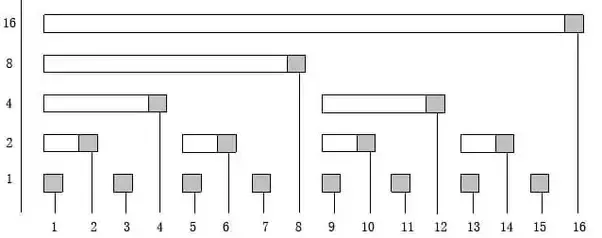
\includegraphics[width=0.6\textwidth]{img/BIT.png}
    \end{frame}

    \begin{frame}{update}
        \begin{itemize}
            \item 如果我們要更改 $A_i$ 的值,那就需要更改所有包含 $i$ 的陣列
            \item 觀察之後會發現,從 $i$ 開始,每次更改後將 $i$ 加上 $lowbit(i)$
            \item 經過的點就是包含 $i$ 的所有區間
        \end{itemize}
    \end{frame}

    \begin{frame}{query}
        \begin{itemize}
            \item 至於查詢 $1 \sim i$ 的和,則是要避免有重疊的線段
            \item 觀察後,會發現其實就是不斷 $- lowbit(i)$
            \item OK!我們會 BIT 了
        \end{itemize}
    \end{frame}

    \begin{frame}{先來個簡單的}
        \begin{block}{\href{https://cses.fi/problemset/task/1648}{CSES Dynamic Range Sum Queries}}
            請寫出一支程式,支援以下操作:\\
            \begin{itemize}
                \item update(i, x):將 $A_i$ 加上 $x$
                \item query(l, r):查詢 $A_l, A_{l+1}, \cdots, A_r$ 的總和
            \end{itemize}
        \end{block}
    \end{frame}

    \begin{frame}{BIT 應用在 LIS 上}
        \begin{itemize}
            \item<1-> BIT 也可以拿來計算最大值
            \item<2-> 我們將 BIT 的區間定義成以該區間內的數字為結尾的 LIS 長度
            \item<3-> 也就是 query(i) 會回傳以 $1 \sim i$ 為結尾的最大 LIS 長度
            \item<4-> 假設這是 tmp,那我們在 tmp 之後就能再接上 $i$,使得 LIS 長度加一
            \item<5-> 如此一來,我們就可以使用 BIT 來計算 LIS 了!
        \end{itemize}
    \end{frame}

    \begin{frame}{最終步驟}
        \begin{enumerate}
            \item 對於每個數字 $a_i$,查詢 tmp = query($a_i$ - 1)
            \item update($a_i$, tmp + 1)
            \item 最後 query(夠大的數字) 就是答案!
        \end{enumerate}
    \end{frame}

    \begin{frame}{逆序數對}
        \begin{block}{\href{https://tioj.ck.tp.edu.tw/problems/1080}{TIOJ 1080 A.逆序數對}}
            計算符合以下條件的數對數量:$i < j, a_i > a_j$
        \end{block}

        \begin{itemize}
            \item<1-> 這題其實是分治的題目
            \item<2-> 但我們可以很開心的用 BIT 解決
            \item<3-> 將 query 設定為數字 $1 \sim i$ 出現的次數
            \item<4-> 對於某個數字 $a_j$,$a_i > a_j$ 的數量就是 n - query($a_j$)
        \end{itemize}
    \end{frame}

    \section{DAG DP}

    \begin{frame}{DAG}
        \begin{itemize}
            \item 不確定圖論有沒有講過
            \item DAG:有向無環圖
            \item 能夠拓樸排序的就是 DAG
        \end{itemize}
    \end{frame}

    \begin{frame}{DAG DP}
        \begin{itemize}
            \item 回想一下第一堂 DP 課,講 Bottom Up 的地方
            \item 有提到 "需要知道轉移點的前後順序"
            \item 有沒有覺得,這跟某種圖論技巧有關呢?
        \end{itemize}
    \end{frame}

    \begin{frame}{Topo Sort}
        \begin{itemize}
            \item<1-> 回想一下,拓樸排序的作用是甚麼?
            \item<2-> 構造出一個順序,使得所有邊都是由這個順序的前面指向後面
            \item<3-> 其實這就跟轉移點的前後順序一樣!
            \item<4-> 將轉移點之間的關係畫成圖,迴圈的順序便是拓樸排序了
            \item<5-> 有了一定的順序,就能夠拿來 DP
        \end{itemize}
    \end{frame}

    \begin{frame}{DAG DP}
        \begin{block}{\href{https://atcoder.jp/contests/dp/tasks/dp_g}{AtCoder DP Contest G - Longest Path}}
            給 DAG,求出一條最長的路徑
        \end{block}

        \begin{itemize}
            \item<1-> 首先,最長路徑有甚麼性質?
            \item<2-> 一定是入度為 0 的點開始,如何證明?
            \item<3-> 若最長路徑的起點 $v$ 入度 $\neq 0$,那麼一定有一個點 $u$ 能夠通到 $v$,那 $v$ 就不可能是起點了
            \item<4-> 由反證法得證
        \end{itemize}
    \end{frame}

    \begin{frame}{DAG DP}
        \begin{block}{\href{https://atcoder.jp/contests/dp/tasks/dp_g}{AtCoder DP Contest G - Longest Path}}
            給 DAG,求出一條最長的路徑
        \end{block}

        \begin{itemize}
            \item<1-> 接著回到 DP
            \item<2-> 狀態很好訂:$dp_i$:以 $i$ 為結尾的最大路徑長度
            \item<3-> 接著來找轉移點,應該也很好想,就是所有通向 $i$ 的邊
            \item<4-> 轉移式:$dp_i = \max(dp_j + 1)$ ($j$ 表所有能連向 $i$ 的邊) 
            \item<5-> 最後,利用 Topo Sort 的順序依序轉移,最後取最大的 $dp_i$ 就是答案!
            \item<6-> 其實這題也有只使用 DFS 的作法,大家可以想想看
        \end{itemize}
    \end{frame}

    \begin{frame}{利用 DP 紀錄路徑}
        \begin{block}{\href{https://cses.fi/problemset/task/1680/}{CSES Longest Flight Route}}
            跟 AtCoder DP Contest G 類似,但是要求出一組解
        \end{block}

        \begin{itemize}
            \item<1-> 我們已經知道怎麼算長度了,那路徑怎麼算呢?
            \item<2-> 還記得子序列 DP 的構造解嗎?
            \item<2-> 我們在子序列 DP 那邊會利用紀錄轉移點來得到構造解,在這裡也可以用!
            \item<3-> $pre_i$:$i$ 的轉移點
            \item<4-> 在拓樸排序的過程中更新 $pre_i$,最後再把這些點連起來就是答案了
        \end{itemize}
    \end{frame}
    
    \begin{frame}{例題}
        \begin{block}{\href{https://atcoder.jp/contests/dp/tasks/dp_g}{AtCoder DP Contest G - Longest Path}}
            給 DAG,求出一條最長的路徑
        \end{block}

        \begin{block}{\href{https://cses.fi/problemset/task/1674/}{CSES https://cses.fi/problemset/task/1674/}}
            共有 $n$ 人,第 $1$ 人是老闆,其餘每個人都有一個上司,求每個人的所有下屬數量
        \end{block}

        \begin{block}{\href{https://cses.fi/problemset/task/1680/}{CSES Longest Flight Route}}
            跟 AtCoder DP Contest G 類似,但是要求出一組解
        \end{block}
    \end{frame}

    \section{樹 DP}

    \begin{frame}{樹 DP}
        \begin{itemize}
            \item 樹其實就是一種 DAG,有些樹 DP 也可以用 DAG 實作(如果樹是有向的),不過這邊我會主要以 DFS 的方式實作
            \item 複習一下樹的術語:
            \begin{itemize}
                \item root:樹根,樹的最頂端
                \item child:子節點,某個點往下一層的點
                \item sub-tree:子樹,由子節點組成的樹
                \item depth:深度,從 root 到某個點的距離
            \end{itemize}
        \end{itemize}
    \end{frame}

    \begin{frame}{樹直徑}
        \begin{itemize}
            \item<1-> 樹直徑:樹上最長的那條路徑
            \item<2-> 假設有一條路徑是以 $i$ 為中心,往 $i$ 的兩條子樹延伸
            \item<3-> 怎樣會最長?
            \item<4-> 從 $i$ 的子節點裡,找出能夠延伸到最長的兩個路徑
        \end{itemize}
    \end{frame}

    \begin{frame}{樹直徑}
        \begin{itemize}
            \item<1-> 假設 $dp_i$ 為以 $i$ 為中心的最大長度
            \item<2-> 那我們會需要幾種東西:
            \begin{itemize}
                \item<2-> $dep_i$:$i$ 的深度
                \item<2-> $sub_i$:$i$ 的子樹中最深的點
            \end{itemize} 
            \item<3-> 那麼 $dp_i$ 怎麼算?
            \item<4-> 假設 $v$ 是 $i$ 的子樹,而其中擁有最大 $sub$ 的兩個點是 $a, b$,那麼 $dp_i$ = $sub_a + sub_b - 2 \cdot dep_i$
            \item<5-> 至於 $sub_i$ 怎麼算呢?簡單,把 $dep$ 當作 DFS 的回傳值,或是直接記錄在陣列裡,就可以收集到所有子樹的資料了!
        \end{itemize}
    \end{frame}

    \begin{frame}{例題}
        \begin{block}{\href{https://cses.fi/problemset/task/1131}{CSES Tree Diameter}}
            求樹直徑
        \end{block}

        \begin{block}{\href{https://tioj.ck.tp.edu.tw/problems/1213}{TIOJ https://tioj.ck.tp.edu.tw/problems/1213}}
            求有權重的樹直徑
        \end{block}

        \begin{block}{\href{https://tioj.ck.tp.edu.tw/problems/2189}{2022 TOIP B. 建設人工島}}
            見原題
        \end{block}
    \end{frame}

    \begin{frame}{其他樹 DP}
        \begin{block}{APCS 202007 P4. 病毒演化}
            有 $n$ 種病毒,每個病毒由一個長度為 $m$ 的 RNA 序列組成,包含 A、U、C、G、@(@ 代表不確定)\\
            除了原始病毒外,所有病毒都是由某個病毒演化而來的,
            求將 $@$ 填入某個字元後,每個病毒與它演化來源的病毒的距離總合最小值是多少?(距離指的是不一樣的位置數)
        \end{block}

        \begin{itemize}
            \item<1-> 狀態可以怎麼訂?我們先將字元編號:AUCG@ 對應 01234(後面會以 $s_{i, j}$ = 0/1/2/3/4 表示)
            \item<2-> $dp_{i, j, k}$:第 $i$ 個病毒,第 $j$ 個位置,第 $k$ 種字元的最小距離
            \item<3-> 對於每個 RNA 序列,我們需要先做一些操作:
            \begin{itemize}
                \item<4-> $dp_{i, j, k} = \begin{cases}
                    0 & \text{if } s_{i, j} = k \text{ or } s_{i, j} = 4 \\
                    \infty & \text{otherwise}
                \end{cases}$
            \end{itemize}
        \end{itemize}
    \end{frame}

    \begin{frame}{其他樹 DP}
        \begin{block}{APCS 202007 P4. 病毒演化}
            有 $n$ 種病毒,每個病毒由一個長度為 $m$ 的 RNA 序列組成,包含 A、U、C、G、@(@ 代表不確定)\\
            除了原始病毒外,所有病毒都是由某個病毒演化而來的,
            求將 $@$ 填入某個字元後,每個病毒與它演化來源的病毒的距離總合最小值是多少?(距離指的是不一樣的位置數)
        \end{block}

        \begin{itemize}
            \item<1-> 至於轉移式怎麼訂呢?
            \item<2-> 對於轉移點 $v$,我們枚舉 $k, l = 0 \sim 4$,如果 $k \neq l$ 就代表要 $+1$
            \item<3-> 最終轉移式:$dp_{i, j, k} =
                \sum\min_{l = 0}^{4}(dp_{v, j, l} + (k \neq l))$
        \end{itemize}
    \end{frame}

    \begin{frame}{例題}
        \begin{block}{APCS 202007 P4. 病毒演化}
            有 $n$ 種病毒,每個病毒由一個長度為 $m$ 的 RNA 序列組成,包含 A、U、C、G、@(@ 代表不確定)\\
            除了原始病毒外,所有病毒都是由某個病毒演化而來的,
            求將 $@$ 填入某個字元後,每個病毒與它演化來源的病毒的距離總合最小值是多少?(距離指的是不一樣的位置數)
        \end{block}
        \begin{itemize}
            \item \href{https://cses.fi/problemset/task/1130}{CSES Tree Matching}
            \item \href{https://codeforces.com/problemset/problem/1528/A}{CF 1528A. Parsa's Humongous Tree}
        \end{itemize}
    \end{frame}

\end{document}